\documentclass{beamer}
\usepackage[utf8]{inputenc}
\usepackage{amsmath}
\usepackage{amsfonts}
\usepackage{amssymb}
\usepackage{empheq}
\usepackage{tikz}
\usepackage{changepage}
\usetikzlibrary{automata, positioning, shapes, arrows}

%Information to be included in the title page:
\title{Combinatorics of Integer Partitions}
\author{Ethan Jensen \\
\small Corban Harwood (Advisor)}
\institute{George Fox University}
\date{February 29, 2020}

\begin{document}
\definecolor{mycolor1}{RGB}{230,230,230}
\definecolor{mycolor2}{RGB}{210,210,210}
\definecolor{mycolor3}{RGB}{190,190,190}

\frame{\titlepage}

\begin{frame}
  \frametitle{Objective}
  \[\frac{1}{1^2} + \frac{1}{2^2} + \frac{1}{3^2} + \frac{1}{4^2}...=\frac{\pi^2}{6}\]
  \newline
  \newline
  \[\zeta(s) = \frac{1}{1^s} + \frac{1}{2^s} + \frac{1}{3^s} + \frac{1}{4^s}...\]
  \newline
  \[\zeta(2) = \frac{\pi^2}{6}\]
  \newline
  What about \(\zeta(4), \zeta(6), \zeta(8)\)?
\end{frame}

\begin{frame}
  \frametitle{Current Methods}
  \[\frac{1}{2q+1}=\sum_{k=1}^s\frac{(-1)^{k+1}2^{k+1}(1-2^{1-2k})q!}{(2q-2k+1)(q-k)!\pi^{2k}}\zeta(2k)\]
  \newline
  \[\sum_{n=0}^{\infty}\zeta(2n)x^{2n} = \frac{-\pi x}{2}\cot{\pi x}\]
  \newline
  \[\zeta(2n) = \frac{B_{2n}(2\pi)^{2n}(-1)^{n+1}}{2(2n)!}\]
  \newline
  \newline
  Is there a better way to calculate \(\zeta(2n)\)?
\end{frame}

\begin{frame}
\frametitle{Outline}
\tableofcontents
\end{frame}

\section{Introduction to Partitions}

\begin{frame}
\frametitle{What is a Partition?}
\[4=1+1+1+1=1+1+2=1+3=2+2=4\]
\newline \newline \newline \newline
The collection C of partitions of 4 is
\[C = \{(1,1,1,1),\ (1,1,2),\ (1,3),\ (2,2),\ (4)\}\]
\newline \newline
\(\lambda = (1,1,2) \textup{ is a partition of 4.}\)
\end{frame}

\begin{frame}
\frametitle{Partitions of Sequences}
\[(2) + (3) = (1+1)+(1+1+1) = (1+1) + (3) = (1+1) + (1+2) = \]
\[(1+1) + (3) = (2) + (1+2) = (2) + (3)\]
\newline \newline \newline
The collection C of partitions of \((2,3)\) is
\[C=\{(1,1,1,1,1),\ (1,1,3),\ (1,1,1,2),\ (1,1,3),\ (1,2,2),\ (2,3)\}\]
\newline
\newline
\((1,1,1,2) \textup{ is \textbf{finer} than } (2,3)\)
\end{frame}

\begin{frame}
\frametitle{Recombining a Partition}
\textit{"Putting Humpty Dumpty back together again"}
\newline \newline
The collection C of recombinations of \((1,1,3)\) is
\[C = \{(1,1,3),\ (2,3),\ (1,4),\ (5)\}\]
\newline
If we counted the number of ways we recombined...
\[C = \{(1,1,3)_2,\ (2,3)_1,\ (1,4)_2,\ (5)_1\}\]
\newline
\newline
\((1,4) \textup{ is coarser than } (1,1,3)\)
\end{frame}

\section{Partitions of Integer Lattices}

\begin{frame}
  \frametitle{Partitioning Integer Lattices}
  Consider the Positive Integer lattices in N-Space:
  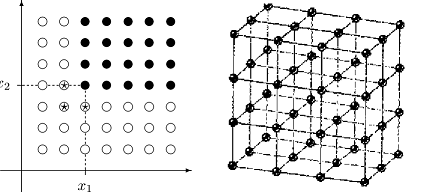
\includegraphics{lattices}
  \newline
  We can partition sets the same way we can partition numbers and sequences.
  \newline \newline
  Partition this set based on the groups of numbers in the sequence that are the same.
  \newline \newline
  We want the tuple \((1,2,3)\) to be in a different set from \((7,2,2)\).
\end{frame}

\begin{frame}
  \frametitle{Partitions as Elementhood Conditions}
  Partition sets: \(S(\lambda)\).
  \newline \newline
  A function that takes in a partition and outputs a set.
  \newline \newline
  Constructed a set using the partition as an instruction, making groups of equal elements.
  \newline \newline
  Here are some elements in the set \(S(2,3)\).
  \[(1,1,2,2,2), (4,3,4,3,4), (3,3,1,3,1), (56, 2, 2, 2, 56), (5,5,5,5,5)\]
  Here are some elements that are not in the set \(S(2,3)\).
  \[(1,2,3,4,5), (2,2,2,2,6), (3,5,3,5,7)\]
\end{frame}

\begin{frame}
  \frametitle{Minimal Partition Sets}
  Consider the set \(S(1,1,1) = \mathbb{Z}_+^3\).
  \newline
  Possible kinds of points:
  \[(a,b,c), (a,c,b), (b,a,c), (b,c,a), (c,a,b), (c,b,a)\]
  \[(a,a,b), (a,b,a), (b,a,a)\]
  \[(a,a,a)\]
  \newline
  For each case, we can assign a new set that only contains points of that shape.
  \newline \newline
  We denote minimal partition sets as \(S'(\boldsymbol{\lambda})\)
\end{frame}

\begin{frame}
  \frametitle{Full Parititions}
  Consider the recombination set C of \((1,1,1)\).
  \[C = \{(1,1,1)_6,\ (1,2)_3,\ (3)_1\}\]
  \[\mathbb{Z}_+^3 = S(1,1,1) = S'(1,1,1)_6 \cup S'(1,2)_3 \cup S'(3)_1\]
  \newline \newline \newline \newline
  \textbf{How many ways are there to combine elements of a given partion to make a different coarser partition?}
\end{frame}

\section{Blocks and Holes}
\begin{frame}
  \frametitle{Blocks and Holes}
  Counting ways to combine elements of a partition into a coarser partition has a physical analogy. \newline
  It is called the \textbf{Blocks and Holes Problem}.
  \newline \newline
  How many different ways are there to distribute the blocks into the holes?
  \begin{figure}[ht]
  	\centering % centers the figure
  	\begin{tikzpicture}[inner sep=3mm]
  \node[draw,fill=mycolor1] (B1) at (0,0) {};
  \node[draw,fill=mycolor1] (B2) at (1,0) {};
  \node[draw,fill=mycolor1] (B3) at (2,0) {};
  \node[draw,fill=mycolor1] (B4) at (2,0.6) {};
  \node[] (L1) at (0,-0.6) {$B_1$};
  \node[] (L1) at (1,-0.6) {$B_2$};
  \node[] (L1) at (2,-0.6) {$B_3$};
  \node[] (L1) at (1,1.8) {Blocks};
  \node[] (L1) at (4.5,1.8) {Holes};
  \node[] (L1) at (4,0) {$H_1$};
  \node[] (L1) at (5,0) {$H_2$};
  \node[draw,fill=mycolor2,dashed] (H1) at (4,-0.6) {};
  \node[draw,fill=mycolor2,dashed] (H2) at (5,-0.6) {};
  \node[draw,fill=mycolor2,dashed] (H3) at (5,-1.2) {};
  \node[draw,fill=mycolor2,dashed] (H4) at (5,-1.8) {};
  \end{tikzpicture}
  	\caption{Blocks and Holes Scenario 1.1}
  \end{figure}
\end{frame}

\begin{frame}
  \frametitle{Blocks and Holes Example}
  \begin{figure}[ht]
  	\centering % centers the figure
  	\begin{tikzpicture}[inner sep=3mm]
  \node[draw,fill=mycolor1] (B1) at (0,0) {};
  \node[draw,fill=mycolor1] (B2) at (1,0) {};
  \node[draw,fill=mycolor1] (B3) at (2,0) {};
  \node[] (B1) at (0,-0.6) {$B_1$};
  \node[] (B2) at (1,-0.6) {$B_2$};
  \node[] (B3) at (2,-0.6) {$B_3$};
  \node[] (T1) at (1,1.8) {Blocks};

  \node[] (H1) at (3.5,0) {$H_1$};
  \node[] (H2) at (4.5,0) {$H_2$};
  \node[] (H3) at (5.5,0) {$H_3$};
  \node[] (T2) at (4.5,1.8) {Holes 1};
  \node[draw,fill=mycolor2,dashed] (H1) at (3.5,-0.6) {};
  \node[draw,fill=mycolor2,dashed] (H2) at (4.5,-0.6) {};
  \node[draw,fill=mycolor2,dashed] (H3) at (5.5,-0.6) {};

  \node[] (H1) at (7,0) {$H_1$};
  \node[] (H2) at (8,0) {$H_2$};
  \node[] (T3) at (7.5,1.8) {Holes 2};

  \node[draw,fill=mycolor2,dashed] (H1) at (7, -0.6) {};
  \node[draw,fill=mycolor2,dashed] (H2) at (8, -0.6) {};
  \node[draw,fill=mycolor2,dashed] (H1) at (8, -1.2) {};

  \node[] (H1) at (9.5, 0) {$H_1$};
  \node[] (T4) at (9.5,1.8) {Holes 3};

  \node[draw,fill=mycolor2,dashed] (H1) at (9.5, -0.6) {};
  \node[draw,fill=mycolor2,dashed] (H2) at (9.5, -1.2) {};
  \node[draw,fill=mycolor2,dashed] (H1) at (9.5, -1.8) {};
 \end{tikzpicture}
  	\caption{Blocks and Holes Scenario 1.2}
  \end{figure}
\end{frame}

\begin{frame}
  \frametitle{Blocks and Holes Solution}
  \begin{figure}[ht]
  	\centering % centers the figure
  	\begin{tikzpicture}[inner sep=3mm]
  \node[draw,fill=mycolor1] (B1) at (0,0) {};
  \node[draw,fill=mycolor1] (B2) at (1,0) {};
  \node[draw,fill=mycolor1] (B3) at (2,0) {};
  \node[] (B1) at (0,0) {$B_1$};
  \node[] (B2) at (1,0) {$B_2$};
  \node[] (B3) at (2,0) {$B_3$};

  \node[draw,fill=mycolor1] (B1) at (3.5,0) {};
  \node[draw,fill=mycolor1] (B2) at (4.5,0) {};
  \node[draw,fill=mycolor1] (B3) at (5.5,0) {};
  \node[] (B1) at (3.5,0) {$B_1$};
  \node[] (B2) at (4.5,0) {$B_3$};
  \node[] (B3) at (5.5,0) {$B_2$};

  \node[draw,fill=mycolor1] (B1) at (7,0) {};
  \node[draw,fill=mycolor1] (B2) at (8,0) {};
  \node[draw,fill=mycolor1] (B3) at (9,0) {};
  \node[] (B1) at (7,0) {$B_2$};
  \node[] (B2) at (8,0) {$B_1$};
  \node[] (B3) at (9,0) {$B_3$};

  \node[draw,fill=mycolor1] (B1) at (0,1) {};
  \node[draw,fill=mycolor1] (B2) at (1,1) {};
  \node[draw,fill=mycolor1] (B3) at (2,1) {};
  \node[] (B1) at (0,1) {$B_2$};
  \node[] (B2) at (1,1) {$B_3$};
  \node[] (B3) at (2,1) {$B_1$};

  \node[draw,fill=mycolor1] (B1) at (3.5,1) {};
  \node[draw,fill=mycolor1] (B2) at (4.5,1) {};
  \node[draw,fill=mycolor1] (B3) at (5.5,1) {};
  \node[] (B1) at (3.5,1) {$B_3$};
  \node[] (B2) at (4.5,1) {$B_1$};
  \node[] (B3) at (5.5,1) {$B_2$};

  \node[draw,fill=mycolor1] (B1) at (7,1) {};
  \node[draw,fill=mycolor1] (B2) at (8,1) {};
  \node[draw,fill=mycolor1] (B3) at (9,1) {};
  \node[] (B1) at (7,1) {$B_3$};
  \node[] (B2) at (8,1) {$B_2$};
  \node[] (B3) at (9,1) {$B_1$};

  \node[draw,fill=mycolor1] (B1) at (0,-1.5) {};
  \node[draw,fill=mycolor1] (B2) at (1,-1.5) {};
  \node[draw,fill=mycolor1] (B3) at (1,-2.1) {};
  \node[] (B1) at (0,-1.5) {$B_1$};
  \node[] (B2) at (1,-1.5) {$B_2$};
  \node[] (B3) at (1,-2.1) {$B_3$};

  \node[draw,fill=mycolor1] (B1) at (2.5,-1.5) {};
  \node[draw,fill=mycolor1] (B2) at (3.5,-1.5) {};
  \node[draw,fill=mycolor1] (B3) at (3.5,-2.1) {};
  \node[] (B1) at (2.5,-1.5) {$B_2$};
  \node[] (B2) at (3.5,-1.5) {$B_1$};
  \node[] (B3) at (3.5,-2.1) {$B_3$};

  \node[draw,fill=mycolor1] (B1) at (5,-1.5) {};
  \node[draw,fill=mycolor1] (B2) at (6,-1.5) {};
  \node[draw,fill=mycolor1] (B3) at (6,-2.1) {};
  \node[] (B1) at (5,-1.5) {$B_3$};
  \node[] (B2) at (6,-1.5) {$B_1$};
  \node[] (B3) at (6,-2.1) {$B_2$};

  \node[draw,fill=mycolor1] (B1) at (8.5,-1.5) {};
  \node[draw,fill=mycolor1] (B2) at (8.5,-2.1) {};
  \node[draw,fill=mycolor1] (B3) at (8.5,-2.7) {};
  \node[] (B1) at (8.5,-1.5) {$B_1$};
  \node[] (B2) at (8.5,-2.1) {$B_2$};
  \node[] (B3) at (8.5,-2.7) {$B_3$};
 \end{tikzpicture}
  	\caption{Blocks and Holes Scenario 1.2}
  \end{figure}
  This solution to the given blocks and holes problem demonstrates that
    \[S(1,1,1) = S'(1,1,1)_6 \cup S'(1,2)_3 \cup S'(3)_1\]
\end{frame}

\section{Applications of Integer Partitions}

\begin{frame}
  \frametitle{Summing over a Partition}
Let \(\boldsymbol{\lambda}\) be a partition of an integer lattice.
\newline
Let \textbf{X} be some tuple \(\textbf{X}=(x_1,x_2,...x_n)\)
\newline
Define a new function D such that
\[D(\boldsymbol{\lambda}) = \sum_{\textbf{X}\in S(\boldsymbol{\lambda})}\prod_{x_i \in \textbf{X}}x_i^{-2}\ \ \ D'(\boldsymbol{\lambda}) = \sum_{\textbf{X}\in S'(\boldsymbol{\lambda})}\prod_{x_i \in \textbf{X}}x_i^{-2}\]
Because D is linear \textbf{and} multiplicative!
\[D(\boldsymbol{\lambda}) = \sum_{ \boldsymbol{\lambda} \vdash \lambda_i}a_iD'(\lambda_i)\]
where \(a_i\) is the number of ways to combine \(\boldsymbol{\lambda}\) into \(\lambda_i\).
\newline \newline
\[D(\lambda_a|\lambda_b) = D{(\lambda_a)}D{(\lambda_b)}\]
where \(\lambda_a|\lambda_b = ({\lambda_a}_1,{\lambda_a}_2,...{\lambda_a}_k,{\lambda_b}_1,{\lambda_b}_2...{\lambda_b}_j)\)
\end{frame}

\begin{frame}
  \frametitle{Solution to the Basel Problem}
  \newline \newline
  Comparing the Maclaurin series of \(\sinh(x)\) with it's Euler product, by a simple calculation we have that
  \[\frac{\sinh(\pi x)}{\pi x} = 1 + \frac{\pi^2x^2}{3!}+\frac{\pi^4x^4}{5!}+\frac{\pi^6x^6}{7!}...=\left(1+\frac{x^2}{1^2}\right)\left(1+\frac{x^2}{2^2}\right)\left(1+\frac{x^2}{3^2}\right)...\]
  By calculating the coefficient of degree 2, we must consider all the ways we can generate terms of degree 2 from the product.
  \[\frac{1}{1^2} + \frac{1}{2^2} + \frac{1}{3^2} + \frac{1}{4^2} + \frac{1}{5^2}... = \frac{\pi^2}{6}\]
  \newline
  What if we want to calculate higher power sums?
  \[\frac{1}{1^4} + \frac{1}{2^4} + \frac{1}{3^4} + \frac{1}{4^4}... = ?\]
\end{frame}

\begin{frame}
  \frametitle{Connection to Particular Zeta Values}
  Consider the following equation we derived earlier.
    \[1 + \frac{\pi^2x^2}{3!}+\frac{\pi^4x^4}{5!}+\frac{\pi^6x^6}{7!}...=\left(1+\frac{x^2}{1^2}\right)\left(1+\frac{x^2}{2^2}\right)\left(1+\frac{x^2}{3^2}\right)...\]
    The term of coefficient of degree 4 is just \(D'(1,1)\).
    \newline
    \[D'(1,1) = \frac{\pi^4}{5!} = \frac{\pi^4}{120}\]
    \newline
    We now have a way to calculate a bunch of the values for the D function.
  \[D'(\overbrace{1,1,1,1...1}^{n}) = \frac{\pi^{2n}}{(2n+1)!}\]
\end{frame}

\begin{frame}
  \frametitle{A Quick Example}
  \begin{figure}[ht]
  	\centering % centers the figure
  	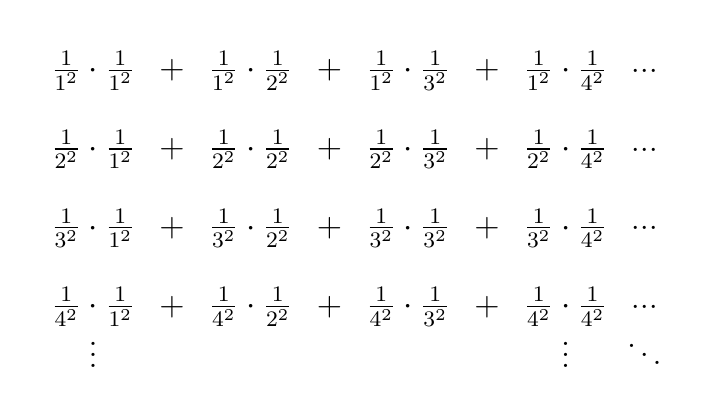
\begin{tikzpicture}[inner sep=3mm]
  	\node[] (L1) at (0,0) {\large $\frac{1}{4^2}\cdot\frac{1}{1^2}$};
  	\node[] (L2) at (1,0) {\large $+$};
  	\node[] (L1) at (2,0) {\large $\frac{1}{4^2}\cdot\frac{1}{2^2}$};
  	\node[] (L2) at (3,0) {\large $+$};
  	\node[] (L1) at (4,0) {\large $\frac{1}{4^2}\cdot\frac{1}{3^2}$};
  	\node[] (L2) at (5,0) {\large $+$};
  	\node[] (L1) at (6,0) {\large $\frac{1}{4^2}\cdot\frac{1}{4^2}$};
  	\node[] (L2) at (7,0) {\large $...$};

  	\node[] (L1) at (0,1) {\large $\frac{1}{3^2}\cdot\frac{1}{1^2}$};
  	\node[] (L2) at (1,1) {\large $+$};
  	\node[] (L1) at (2,1) {\large $\frac{1}{3^2}\cdot\frac{1}{2^2}$};
  	\node[] (L2) at (3,1) {\large $+$};
  	\node[] (L1) at (4,1) {\large $\frac{1}{3^2}\cdot\frac{1}{3^2}$};
  	\node[] (L2) at (5,1) {\large $+$};
  	\node[] (L1) at (6,1) {\large $\frac{1}{3^2}\cdot\frac{1}{4^2}$};
  	\node[] (L2) at (7,1) {\large $...$};

  	\node[] (L1) at (0,2) {\large $\frac{1}{2^2}\cdot\frac{1}{1^2}$};
  	\node[] (L2) at (1,2) {\large $+$};
  	\node[] (L1) at (2,2) {\large $\frac{1}{2^2}\cdot\frac{1}{2^2}$};
  	\node[] (L2) at (3,2) {\large $+$};
  	\node[] (L1) at (4,2) {\large $\frac{1}{2^2}\cdot\frac{1}{3^2}$};
  	\node[] (L2) at (5,2) {\large $+$};
  	\node[] (L1) at (6,2) {\large $\frac{1}{2^2}\cdot\frac{1}{4^2}$};
  	\node[] (L2) at (7,2) {\large $...$};

  	\node[] (L1) at (0,3) {\large $\frac{1}{1^2}\cdot\frac{1}{1^2}$};
  	\node[] (L2) at (1,3) {\large $+$};
  	\node[] (L1) at (2,3) {\large $\frac{1}{1^2}\cdot\frac{1}{2^2}$};
  	\node[] (L2) at (3,3) {\large $+$};
  	\node[] (L1) at (4,3) {\large $\frac{1}{1^2}\cdot\frac{1}{3^2}$};
  	\node[] (L2) at (5,3) {\large $+$};
  	\node[] (L1) at (6,3) {\large $\frac{1}{1^2}\cdot\frac{1}{4^2}$};
  	\node[] (L2) at (7,3) {\large $...$};

  	\node[] (L3) at (0,-0.5) {\large $\vdots$};
  	\node[] (L3) at (6,-0.5) {\large $\vdots$};
  	\node[] (L3) at (7,-0.5) {\large $\ddots$};
  	\end{tikzpicture}
  	\caption{Addition Square}
  \end{figure}
  Going row by row, we have that this sum is equal to
  \[\left(\frac{1}{1^2} + \frac{1}{2^2} + \frac{1}{3^2}...\right)\left(\frac{1}{1^2} + \frac{1}{2^2} + \frac{1}{3^2}...\right) = \left(\frac{\pi^2}{6}\right)^2 = \frac{\pi^4}{36}\]
\end{frame}

\begin{frame}
  \frametitle{A Quick Example Part }
  \begin{figure}[ht]
  	\centering % centers the figure
  	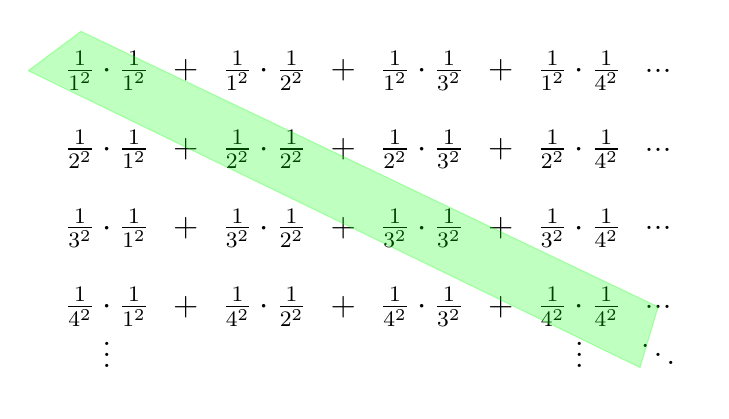
\begin{tikzpicture}[inner sep=3mm]
  	\node[] (L1) at (0,0) {\large $\frac{1}{4^2}\cdot\frac{1}{1^2}$};
  	\node[] (L2) at (1,0) {\large $+$};
  	\node[] (L1) at (2,0) {\large $\frac{1}{4^2}\cdot\frac{1}{2^2}$};
  	\node[] (L2) at (3,0) {\large $+$};
  	\node[] (L1) at (4,0) {\large $\frac{1}{4^2}\cdot\frac{1}{3^2}$};
  	\node[] (L2) at (5,0) {\large $+$};
  	\node[] (L1) at (6,0) {\large $\frac{1}{4^2}\cdot\frac{1}{4^2}$};
  	\node[] (L2) at (7,0) {\large $...$};

  	\node[] (L1) at (0,1) {\large $\frac{1}{3^2}\cdot\frac{1}{1^2}$};
  	\node[] (L2) at (1,1) {\large $+$};
  	\node[] (L1) at (2,1) {\large $\frac{1}{3^2}\cdot\frac{1}{2^2}$};
  	\node[] (L2) at (3,1) {\large $+$};
  	\node[] (L1) at (4,1) {\large $\frac{1}{3^2}\cdot\frac{1}{3^2}$};
  	\node[] (L2) at (5,1) {\large $+$};
  	\node[] (L1) at (6,1) {\large $\frac{1}{3^2}\cdot\frac{1}{4^2}$};
  	\node[] (L2) at (7,1) {\large $...$};

  	\node[] (L1) at (0,2) {\large $\frac{1}{2^2}\cdot\frac{1}{1^2}$};
  	\node[] (L2) at (1,2) {\large $+$};
  	\node[] (L1) at (2,2) {\large $\frac{1}{2^2}\cdot\frac{1}{2^2}$};
  	\node[] (L2) at (3,2) {\large $+$};
  	\node[] (L1) at (4,2) {\large $\frac{1}{2^2}\cdot\frac{1}{3^2}$};
  	\node[] (L2) at (5,2) {\large $+$};
  	\node[] (L1) at (6,2) {\large $\frac{1}{2^2}\cdot\frac{1}{4^2}$};
  	\node[] (L2) at (7,2) {\large $...$};

  	\node[] (L1) at (0,3) {\large $\frac{1}{1^2}\cdot\frac{1}{1^2}$};
  	\node[] (L2) at (1,3) {\large $+$};
  	\node[] (L1) at (2,3) {\large $\frac{1}{1^2}\cdot\frac{1}{2^2}$};
  	\node[] (L2) at (3,3) {\large $+$};
  	\node[] (L1) at (4,3) {\large $\frac{1}{1^2}\cdot\frac{1}{3^2}$};
  	\node[] (L2) at (5,3) {\large $+$};
  	\node[] (L1) at (6,3) {\large $\frac{1}{1^2}\cdot\frac{1}{4^2}$};
  	\node[] (L2) at (7,3) {\large $...$};

  	\node[] (L3) at (0,-0.5) {\large $\vdots$};
  	\node[] (L3) at (6,-0.5) {\large $\vdots$};
  	\node[] (L3) at (7,-0.5) {\large $\ddots$};

    \filldraw [green, opacity = 0.25] (-1,3) -- (6.77, -0.77) -- (7, 0) -- (-0.33, 3.5) -- (-1,3);
  	\end{tikzpicture}
  	\caption{Addition Square}
  \end{figure}
  Looking at the partition, we have that this sum is equal to
  \[D'(1,1) + \left(\frac{1}{1^4} + \frac{1}{2^4} + \frac{1}{3^4} + \frac{1}{4^4}\right)\]
\end{frame}

\begin{frame}
  \frametitle{Calculating Subsequent Zeta Values}
  The collection C of recombinations of (1,1) is
  \[C = \{(1,1)_2,\ (2)_1\}\]
  It follows that
  \[D(1,1) = 2D'(1,1) + D'(2)\]
  \[D(1)D(1) = 2D'(1,1) + D(2)\]
  \[\zeta(2)^2 = 2D'(1,1) + \zeta(4)\]
  \[\left(\frac{\pi^2}{6}\right)^2=2\frac{\pi^4}{120} + \zeta(4)\]
  \boxed{\therefore \zeta(4) = \frac{\pi^4}{90}}
\end{frame}

\begin{frame}
  \frametitle{Calculating Subsequent Zeta Values cont.}
  \[(1,1,1) \rightarrow \{(1,1,1)_6 +(1,2)_3 + (3)_1\}\]
  \[D(1,1,1) = 6D'(1,1,1) + 3D'(1,2) + D'(3)\]
    \[(1,2) \rightarrow \{(1,2)_1 + (3)_1\}\]
  \[D(1,2) = D'(1,2) + D'(3)\]
  With a quick substitution, we have
  \[D(1,1,1) = 6D'(1,1,1) + 3D(1,2) - 2D'(3)\]
  \[\left(D(1)\right)^3 = 6D'(1,1,1) + 3D(1)D(2) - 2D(3)\]
  \[\frac{\pi^6}{216} = \frac{6\pi^6}{7!} + \frac{3\pi^6}{6\cdot 90} -2\zeta(6)\]
  \[2\zeta(6) = \frac{2\pi^6}{945}\]
  \boxed{\therefore \zeta(6) = \frac{\pi^6}{945}}
\end{frame}

\begin{frame}
  \frametitle{Solving the Blocks and Holes problem}
  Higher dimensions are spicy!
  \begin{figure}[ht]
  	\centering % centers the figure
  	\begin{tikzpicture}[inner sep=3mm]
  \node[draw,fill=mycolor1] (B1) at (0,0) {};
  \node[draw,fill=mycolor1] (B2) at (1,0) {};
  \node[draw,fill=mycolor1] (B3) at (2,0) {};
  \node[draw,fill=mycolor1] (B4) at (2,0.6) {};
  \node[draw, fill=mycolor1] (B5) at (3, 0) {};
  \node[draw, fill=mycolor1] (B5) at (3, 0.6) {};
  \node[draw, fill=mycolor1] (B5) at (3, 1.2) {};
  \node[draw, fill=mycolor1] (B5) at (4, 0) {};
  \node[draw, fill=mycolor1] (B5) at (4, 0.6) {};
  \node[draw, fill=mycolor1] (B5) at (4, 1.2) {};
  \node[] (L1) at (0,-0.6) {$B_1$};
  \node[] (L1) at (1,-0.6) {$B_2$};
  \node[] (L1) at (2,-0.6) {$B_3$};
  \node[] (L1) at (3,-0.6) {$B_4$};
  \node[] (L1) at (4,-0.6) {$B_5$};
  \node[] (L1) at (2,1.8) {Blocks};
  \node[] (L1) at (7.5,1.8) {Holes};
  \node[] (L1) at (6,0) {$H_1$};
  \node[] (L1) at (7,0) {$H_2$};
  \node[] (L1) at (8,0) {$H_3$};
  \node[] (L1) at (9,0) {$H_4$};
  \node[draw,fill=mycolor2,dashed] (H1) at (6,-0.6) {};
  \node[draw,fill=mycolor2,dashed] (H2) at (7,-0.6) {};
  \node[draw,fill=mycolor2,dashed] (H3) at (7,-1.2) {};
  \node[draw,fill=mycolor2,dashed] (H4) at (7,-1.8) {};
  \node[draw,fill=mycolor2,dashed] (H2) at (8,-0.6) {};
  \node[draw,fill=mycolor2,dashed] (H3) at (8,-1.2) {};
  \node[draw,fill=mycolor2,dashed] (H4) at (8,-1.8) {};
  \node[draw,fill=mycolor2,dashed] (H2) at (9,-0.6) {};
  \node[draw,fill=mycolor2,dashed] (H3) at (9,-1.2) {};
  \node[draw,fill=mycolor2,dashed] (H4) at (9,-1.8) {};
  \end{tikzpicture}
  	\caption{Blocks and Holes Scenario 1.1}
  \end{figure}
Use a computer to virtually place blocks into holes.
\end{frame}

\begin{frame}
  \frametitle{The complete algorithm}
  We want to compute \(\zeta(2n)\). \newline \newline
  We can use the blocks and holes algorithm to build a system of equations. \newline \newline
  After solving the system of equations we can use the master equation and recursion to solve for \(\zeta(2n)\).
\end{frame}

\begin{frame}
\frametitle{Conclusion}
\textbf{(1)} Partitions
\newline \newline
\textbf{(2)} Recombinations of Partitions
\newline \newline
\textbf{(3)} Partitions of Integer Lattices
\newline \newline
\textbf{(4)} The D function
\newline \newline
\textbf{(5)} Specifying the combinatorics problem.
\newline \newline
\textbf{(5)} Calculating Positive even Zeta values recursively
\end{frame}

\begin{frame}
\frametitle{The importance of multiplicity of proofs}
Mathematics is about methods - more so than about the Theorems themselves.
Zeta values can be calculated using: \newline
\begin{itemize}
  \item Complex Analysis
  \item Bernoulli numbers
  \item Fourier Series
\end{itemize}
\(\ \)
\newline \newline
My method provides a new way to calculate positive even zeta values without using any heavy mathematical machinery.
\newline \newline
This method is a continuagtion of the work of Leonhard Euler. Basel problem solved in (1734).
\end{frame}

\begin{frame}
  \frametitle{Connections to the Riemann Hypothesis}
  \textit{What is the hardest way to win \$1,000,000?}
  \newline \newline \newline \newline \newline \newline
  Proofs to difficult problems can sometimes arise from seemingly unrelated areas of mathematics.
  \newline \newline
  Chaotic behavior of the primes and the Bernoulli numbers linked to the chaotic behavior of partitions.
  \newline \newline
  This work provides a strong link between Combinatorics and Analytic Number Theory.
\end{frame}

\begin{frame}
  \frametitle{References}
  “Growth and Change in Mathematics.” Understanding Infinity: the Mathematics of Infinite Processes, by A. Gardiner, Dover Publications, 2002, pp. 19–23.
  \newline
  \newline
  Flammable Maths, "The Basel Problem \& its Alternating Formulation [ The Dirichlet Eta Function ]",\textit{YouTube} video, 15:12. Jan. 11, 2019. \newline
  https://www.youtube.com/watch?v=MAoI\_\_hbdWM
  \newline
  \newline
  Flammable Maths, "\textbf{BUT HOW DID EULER DO IT}?! A BEAUTIFUL Solution to the FAMOUS Basel Problem!",\textit{YouTube} video, 18:04. May 24, 2019. https://www.youtube.com/watch?v=JAr512hLsEU
\end{frame}
\end{document}
